%{{第七十一回}}{第七十一回}}

\chapter{嫌隙人有心生嫌隙\hspace{.5em}鸳鸯女无意遇鸳鸯}

{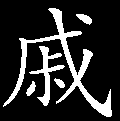
\includegraphics[width=3mm]{../Images/00005}\kaishu 叙贾母开寿诞,与宁府祭宗祠是一样手笔,俱为五凤裁诏体。}

话说贾政回京之后,诸事完毕,赐假一月在家歇息。因年景渐老,事重身衰,又近因在外几年,骨肉离异,今得晏然复聚于庭室,自觉喜幸不尽。一应大小事务一概益发付于度外,只是看书,闷了便与清客们下棋吃酒,或日间在里面母子夫妻共叙天伦庭闱之乐。

因今岁八月初三日乃贾母八旬之庆,又因亲友全来,恐筵宴排设不开,便早同贾赦及贾珍贾琏等商议,议定于七月二十八日起至八月初五日止荣宁两处齐开筵宴,宁国府中单请官客,荣国府中单请堂客,大观园中收拾出缀锦阁并嘉荫堂等几处大地方来作退居。二十八日请皇亲、驸马、王公、诸公主、郡主、王妃、国君、太君、夫人等,二十九日便是阁下、都府、督镇及诰命等,三十日便是诸官长及诰命并远近亲友及堂客。初一日是贾赦的家宴,初二日是贾政,初三日是贾珍贾琏,初四日是贾府中合族长幼大小共凑的家宴。初五日是赖大林之孝等家下管事人等共凑一日。自七月上旬,送寿礼者便络绎不绝。礼部奉旨:钦赐金玉如意一柄,彩缎四端,金玉环四个,帑银五百两。元春又命太监送出金寿星一尊,沉香拐一只,伽南珠一串,福寿香一盒,金锭一对,银锭四对,彩缎十二匹,玉杯四只。馀者自亲王驸马以及大小文武官员之家凡所来往者,莫不有礼,不能胜记。堂屋内设下大桌案,铺了红毡,将凡所有精细之物都摆上,请贾母过目。贾母先一二日还高兴过来瞧瞧,后来烦了,也不过目,只说:“叫凤丫头收了,改日闷了再瞧。”

至二十八日,两府中俱悬灯结彩,屏开鸾凤,褥设芙蓉,笙箫鼓乐之音,通衢越巷。宁府中本日只有北静王、南安郡王、永昌驸马、乐善郡王并几个世交公侯应袭,荣府中南安王太妃、北静王妃并几位世交公侯诰命。贾母等皆是按品大妆迎接。大家厮见,先请入大观园内嘉荫堂,茶毕更衣,方出至荣庆堂上拜寿入席。大家谦逊半日,方才入席。上面两席是南北王妃,下面依叙,便是众公侯诰命。左边下手一席,陪客是锦乡侯诰命与临昌伯诰命,右边下手一席,方是贾母主位。邢夫人王夫人带领尤氏凤姐并族中几个媳妇,两溜雁翅站在贾母身后侍立。林之孝赖大家的带领众媳妇都在竹帘外面侍候上菜上酒,周瑞家的带领几个丫鬟在围屏后侍候呼唤。凡跟来的人,早又有人管待别处去了。

一时台上参了场,台下一色十二个未留发的小厮侍候。须臾,一小厮捧了戏单至阶下,先递与回事的媳妇。这媳妇接了,才递与林之孝家的,用一小茶盘托上,挨身入帘来递与尤氏的侍妾配凤。配凤接了才奉与尤氏。尤氏托着走至上席,南安太妃谦让了一回,点了一出吉庆戏文,然后又谦让了一回,北静王妃也点了一出。众人又让了一回,命随便拣好的唱罢了。少时,菜已四献,汤始一道,跟来各家的放了赏。大家便更衣复入园来,另献好茶。

南安太妃因问宝玉,贾母笑道:“今日几处庙里念‘保安延寿经’,他跪经去了。”又问众小姐们,贾母笑道:“他们姊妹们病的病,弱的弱,见人腼腆,所以叫他们给我看屋子去了。有的是小戏子,传了一班在那边厅上陪着他姨娘家姊妹们也看戏呢。”南安太妃笑道:“既这样,叫人请来。”贾母回头命凤姐儿去把史、薛、林带来,“再只叫你三妹妹陪着来罢。”凤姐答应了,来至贾母这边,只见他姊妹们正吃果子看戏,宝玉也才从庙里跪经回来。凤姐儿说了话。宝钗姊妹与黛玉、探春、湘云五人来至园中,大家见了,不过请安问好让坐等事。众人中也有见过的,还有一两家不曾见过的,都齐声夸赞不绝。{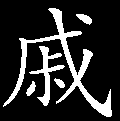
\includegraphics[width=3mm]{../Images/00005}\kaishu 人非草木,见此数人,焉得不垂涎称妙?}\footnote{此批戚、蒙本均混入正文。}其中湘云最熟,南安太妃因笑道:“你在这里,听我来了还不出来,还只等请去。我明儿和你叔叔算账。”因一手拉着探春,一手拉着宝钗,问几岁了,又连声夸赞。因又松了他两个,又拉着黛玉宝琴,也着实细看,极夸一回。又笑道:“都是好的,不知叫我夸那一个的是。”早有人将备用礼物打点出五分来:金玉戒指各五个,腕香珠五串。南安太妃笑道:“你姊妹们别笑话,留着赏丫头们罢。”五人忙拜谢过。北静王妃也有五样礼物,馀者不必细说。

吃了茶,园中略逛了一逛,贾母等因又让入席。南安太妃便告辞,说身上不快,“今日若不来,实在使不得,因此恕我竟先要告别了。”贾母等听说,也不便强留,大家又让了一回,送至园门,坐轿而去。接着北静王妃略一坐也就告辞了。馀者也有终席的,也有不终席的。

贾母劳乏了一日,次日便不会人,一应都是邢夫人王夫人管待。有那些世家子弟拜寿的,只到厅上行礼,贾赦、贾政、贾珍等还礼管待,至宁府坐席。不在话下。

这几日,尤氏晚间也不回那府里去,白日间待客,晚间陪贾母顽笑,又帮着凤姐料理出入大小器皿,以及收放赏礼事务,晚间在园内李氏房中歇宿。这日晚间伏侍过贾母晚饭后,贾母因说:“你们也乏了,我也乏了,早些寻一点子吃的歇歇去。明儿还要起早闹呢。”尤氏答应着退了出来,到凤姐儿房里来吃饭。凤姐儿在楼上看着人收送礼的新围屏,只有平儿在房里与凤姐儿叠衣服。尤氏因问:“你们奶奶吃了饭了没有?”平儿笑道:“吃饭岂不请奶奶去的。”尤氏笑道:“既这样,我别处找吃的去。饿的我受不得了。”说着就走。平儿忙笑道:“奶奶请回来。这里有点心,且点补一点儿,回来再吃饭。”尤氏笑道:“你们忙的这样,我园里和他姊妹们闹去。”一面说,一面就走。平儿留不住,只得罢了。

且说尤氏一径来至园中,只见园中正门与各处角门{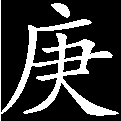
\includegraphics[width=3mm]{../Images/00004}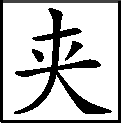
\includegraphics[width=3mm]{../Images/00012}\footnotesize \kaishu 伏下文。}仍未关,犹吊着各色彩灯,因回头命小丫头叫该班的女人。那丫鬟走入班房中,竟没一个人影,回来回了尤氏。尤氏便命传管家的女人。这丫头应了便出去,到二门外鹿顶内,乃是管事的女人议事取齐之所。到了这里,只有两个婆子分菜果呢。因问:“那一位奶奶在这里?东府奶奶立等一位奶奶,有话吩咐。”这两个婆子只顾分菜果,又听见是东府里的奶奶,不大在心上,因就回说:“管家奶奶们才散了。”小丫头道:“散了,你们家里传他去。”婆子道:“我们只管看屋子,不管传人。姑娘要传人再派传人的去。”小丫头听了道:“嗳呀,嗳呀,这可反了!怎么你们不传去?你哄那新来了的,怎么哄起我来了!素日你们不传谁传去!这会子打听了梯己信儿,或是赏了那位管家奶奶的东西,你们争着狗颠儿似的传去的,不知谁是谁呢。琏二奶奶要传,你们可也这么回?”这两个婆子一则吃了酒,二则被这丫头揭挑着弊病,便羞激怒了,因回口道:“扯你的臊!我们的事,传不传不与你相干!你不用揭挑我们,你想想,你那老子娘在那边管家爷们跟前比我们还更会溜呢。什么‘清水下杂面,你吃我也见’的事,各家门,另家户,你有本事,排场你们那边人去。我们这边,你们还早些呢!”丫头听了,气白了脸,因说道:“好,好,这话说的好!”一面转身进来回话。

尤氏已早入园来,因遇见了袭人、宝琴、湘云三人同着地藏庵的两个姑子正说故事顽笑,尤氏因说饿了,先到怡红院,袭人装了几样荤素点心出来与尤氏吃。两个姑子、宝琴、湘云等都吃茶,仍说故事。那小丫头子一径找了来,气狠狠的把方才的话都说了出来。尤氏听了,冷笑道:“这是两个什么人?”两个姑子并宝琴湘云等听了,生怕尤氏生气,忙劝说:“没有的事,必是这一个听错了。”两个姑子笑推这丫头道:“你这孩子好性气,那糊涂老嬷嬷们的话,你也不该来回才是。咱们奶奶万金之躯,劳乏了几日,黄汤辣水没吃,咱们哄他欢喜一会还不得一半儿,说这些话做什么。”袭人也忙笑拉出他去,说:“好妹子,你且出去歇歇,我打发人叫他们去。”尤氏道:“你不要叫人,你去就叫这两个婆子来,到那边把他们家的凤儿叫来。”袭人笑道:“我请去。”尤氏道:“偏不要你去。”两个姑子忙立起身来,笑道:“奶奶素日宽洪大量,今日老祖宗千秋,奶奶生气,岂不惹人谈论。”宝琴湘云二人也都笑劝。尤氏道:“不为老太太的千秋,我断不依。且放着就是了。”

说话之间,袭人早又遣了一个丫头去到园门外找人,可巧遇见周瑞家的,这小丫头子就把这话告诉周瑞家的。周瑞家的虽不管事,因他素日仗着是王夫人的陪房,原有些体面,心性乖滑,专管各处献勤讨好,所以各处房里的主人都喜欢他。他今日听了这话,忙的便跑入怡红院来,一面飞走,一面口内说:“气坏了奶奶了,可了不得!我们家里,如今惯的太不堪了。偏生我不在跟前,若在跟前,且打给他们几个耳刮子,再等过了这几日算账。”尤氏见了他,也便笑道:“周姐姐你来,有个理你说说。这早晚门还大开着,明灯亮烛,出入的人又杂,倘有不防的事,如何使得?因此叫该班的人吹灯关门。谁知一个人芽儿也没有。”周瑞家的道:“这还了得!前儿二奶奶还吩咐了他们,说这几日事多人杂,一晚就关门吹灯,不是园里人不许放进去。今儿就没了人。这事过了这几日,必要打几个才好。”尤氏又说小丫头子的话。周瑞家的道:“奶奶不要生气,等过了事,我告诉管事的打他个臭死。只问他们,谁叫他们说这‘各家门各家户’的话!我已经叫他们吹了灯,关上正门和角门子。”正乱着,只见凤姐儿打发人来请吃饭。尤氏道:“我也不饿了,才吃了几个饽饽,请你奶奶自吃罢。”

一时周瑞家的得便出去,便把方才的事回了凤姐,又说:“这两个婆子就是管家奶奶,时常我们和他说话,都似狠虫一般。奶奶若不戒饬,大奶奶脸上过不去。”凤姐道:“既这么着,记上两人的名字,等过了这几日,捆了送到那府里凭大嫂子开发,或是打几下子,或是他开恩饶了他们,随他去就是了,什么大事。”周瑞家的听了,巴不得一声儿------素日因与这几个人不睦------出来了,便命一个小厮到林之孝家传凤姐的话,立刻叫林之孝家的进来见大奶奶,一面又传人立刻捆起这两个婆子来,交到马圈里派人看守。

林之孝家的不知有什么事,此时已经点灯,忙坐车进来,先见凤姐。至二门上传进话去,丫头们出来说:“奶奶才歇了。大奶奶在园里,叫大娘见了大奶奶就是了。”林之孝家的只得进园来到稻香村,丫鬟们回进去,尤氏听了反过意不去,忙唤进他来,因笑向他道:“我不过为找人找不着因问你,你既去了,也不是什么大事,谁又把你叫进来,倒要你白跑一遭。不大的事,已经撒开手了。”林之孝家的也笑道:“二奶奶打发人传我,说奶奶有话吩咐。”尤氏笑道:“这是那里的话,只当你没去,白问你。这是谁又多事告诉了凤丫头,大约周姐姐说的。家去歇着罢,没有什么大事。”李纨又要说原故,尤氏反拦住了。林之孝家的见如此,只得便回身出园去。可巧遇见赵姨娘,姨娘因笑道:“嗳哟哟,我的嫂子!这会子还不家去歇歇,还跑些什么?”林之孝家的便笑说何曾不家去的,如此这般进来了。又是个齐头故事。赵姨娘原是好察听这些事的,且素日又与管事的女人们扳厚,互相连络,好作首尾。方才之事,已竟闻得八九,听林之孝家的如此说,便恁般如此告诉了林之孝家的一遍,林之孝家的听了,笑道:“原来是这事,也值一个屁!开恩呢,就不理论,心窄些儿,也不过打几下子就完了。”赵姨娘道:“我的嫂子,事虽不大,可见他们太张狂了些。巴巴的传进你来,明明戏弄你,顽算你。快歇歇去,明儿还有事呢,也不留你吃茶去。”

说毕,林之孝家的出来,到了侧门前,就有方才两个婆子的女儿上来哭着求情。林之孝家的笑道:“你这孩子好糊涂,谁叫你娘吃酒混说了,惹出事来,连我也不知道。二奶奶打发人捆他,连我还有不是呢。我替谁讨情去。”这两个小丫头子才七八岁,原不识事,只管哭啼求告。缠的林之孝家的没法,因说道:“糊涂东西!你放着门路不去,却缠我来。你姐姐现给了那边太太作陪房费大娘的儿子,你走过去告诉你姐姐,叫亲家娘和太太一说,什么完不了的事!”一语提醒了这一个,那一个还求。林之孝家的啐道:“糊涂攮的!他过去一说,自然都完了。没有个单放了他妈,又只打你妈的理。”说毕,上车去了。

这一个小丫头果然过来告诉了他姐姐,和费婆子说了。这费婆子原是邢夫人的陪房,起先也曾兴过时,只因贾母近来不大作兴邢夫人,所以连这边的人也减了威势。凡贾政这边有些体面的人,那边各各皆虎视耽耽。这费婆子常倚老卖老,仗着邢夫人,常吃些酒,嘴里胡骂乱怨的出气。如今贾母庆寿这样大事,干看着人家逞才卖技办事,呼幺喝六弄手脚,心中早已不自在,指鸡骂狗,闲言闲语的乱闹。这边的人也不和他较量。如今听了周瑞家的捆了他亲家,越发火上浇油,仗着酒兴,指着隔断的墙{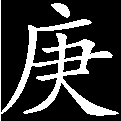
\includegraphics[width=3mm]{../Images/00004}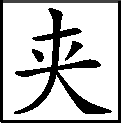
\includegraphics[width=3mm]{../Images/00012}\footnotesize \kaishu 细致之甚。}大骂了一阵,便走上来求邢夫人,说他亲家并没什么不是,“不过和那府里的大奶奶的小丫头白斗了两句话,周瑞家的便调唆了咱家二奶奶捆到马圈里,等过了这两日还要打。求太太------我那亲家娘也是七八十岁的老婆子------和二奶奶说声,饶他这一次罢。”邢夫人自为要鸳鸯之后讨了没意思,后来见贾母越发冷淡了他,凤姐的体面反胜自己,且前日南安太妃来了,要见他姊妹,贾母又只令探春出来,迎春竟似有如无,自己心内早已怨忿不乐,只是使不出来。又值这一干小人在侧,他们心内嫉妒挟怨之事不敢施展,便背地里造言生事,调拨主人。先不过是告那边的奴才,后来渐次告到凤姐“只哄着老太太喜欢了他好就中作威作福,辖治着琏二爷,调唆二太太,把这边的正经太太倒不放在心上。”后来又告到王夫人,说:“老太太不喜欢太太,都是二太太和琏二奶奶调唆的。”邢夫人纵是铁心铜胆的人,妇女家终不免生些嫌隙之心,近日因此着实恶绝凤姐。今听了如此一篇话,也不说长短。

至次日一早,见过贾母,众族中人到齐,坐席开戏。贾母高兴,又见今日无远亲,都是自己族中子侄辈,只便衣常妆出来,堂上受礼。当中独设一榻,引枕靠背脚踏俱全,自己歪在榻上。榻之前后左右,皆是一色的小矮凳,宝钗、宝琴、黛玉、湘云、迎春、探春、惜春姊妹等围绕。因贾㻞之母也带了女儿喜鸾,贾琼之母也带了女儿四姐儿,还有几房的孙女儿,大小共有二十来个。贾母独见喜鸾和四姐儿生得又好,说话行事与众不同,心中喜欢,便命他两个也过来榻前同坐。宝玉却在榻上脚下与贾母捶腿。首席便是薛姨妈,下边两溜皆顺着房头辈数下去。帘外两廊都是族中男客,也依次而坐。

先是那女客一起一起行礼,后方是男客行礼。贾母歪在榻上,只命人说“免了罢”,早已都行完了。然后赖大等带领众家人,从仪门直跪至大厅上,磕头礼毕,又是众家下媳妇,然后各房的丫鬟,足闹了两三顿饭时。然后又抬了许多雀笼来,在当院中放了生。贾赦等焚过了天地寿星纸,方开戏饮酒。直到歇了中台,贾母方进来歇息,命他们取便,因命凤姐儿留下喜鸾四姐儿顽两日再去。凤姐儿出来便和他母亲说,他两个母亲素日都承凤姐的照顾,也巴不得一声儿。他两个也愿意在园内顽耍,至晚便不回家了。

邢夫人直至晚间散时,当着许多人陪笑和凤姐求情说:“我听见昨儿晚上二奶奶生气,打发周管家的娘子捆了两个老婆子,可也不知犯了什么罪。论理我不该讨情,我想老太太好日子,发狠的还舍钱舍米,周贫济老,咱们家先倒折磨起老人家来了。不看我的脸,权且看老太太,竟放了他们罢。”说毕,上车去了。凤姐听了这话,又当着许多人,又羞又气,一时抓寻不着头脑,憋得脸紫涨,回头向赖大家的等笑道:{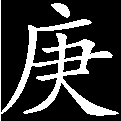
\includegraphics[width=3mm]{../Images/00004}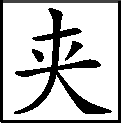
\includegraphics[width=3mm]{../Images/00012}\footnotesize \kaishu 又写笑,妙!凡凤真怒处必曰“笑”,凌凌不错。}\footnote{“凌凌不错”,比较费解。查本书批语中,与“不错”搭配的词语有“一丝”(四处)和“真真”(一处)。按“真真不错”的意思是“确实好”,用在此处不很贴切,而“一丝不错”的意思是“一点也没错”,用在这里正合适。但“凌凌”重字,或当校作“丝丝”。}“这是那里的话。昨儿因为这里的人得罪了那府里的大嫂子,我怕大嫂子多心,所以尽让他发放,并不为得罪了我。这又是谁的耳报神这么快。”王夫人因问为什么事,凤姐儿笑将昨日的事说了。尤氏也笑道:“连我并不知道。你原也太多事了。”凤姐儿道:“我为你脸上过不去,所以等你开发,不过是个礼。就如我在你那里有人得罪了我,你自然送了来尽我。凭他是什么好奴才,到底错不过这个礼去。这又不知谁过去没的献勤儿,这也当作一件事情去说。”王夫人道:“你太太说的是。就是珍哥儿媳妇也不是外人,也不用这些虚礼。老太太的千秋要紧,放了他们为是。”说着,回头便命人去放了那两个婆子。凤姐由不得越想越气越愧,不觉的灰心转悲,滚下泪来。因赌气回房哭泣,又不使人知觉。偏是贾母打发了琥珀来叫立等说话。琥珀见了,诧异道:“好好的,这是什么原故?那里立等你呢。”凤姐听了,忙擦干了泪,洗面另施了脂粉,方同琥珀过来。

贾母因问道:“前儿这些人家送礼来的共有几家有围屏?”凤姐儿道:“共有十六家有围屏,十二架大的,四架小的炕屏。内中只有江南甄家{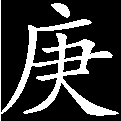
\includegraphics[width=3mm]{../Images/00004}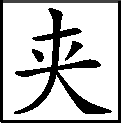
\includegraphics[width=3mm]{../Images/00012}\footnotesize \kaishu 好,一提甄事。{$\diamond$}盖真事欲显,假事将尽。}一架大屏十二扇,大红缎子缂丝‘满床笏’,一面是泥金‘百寿图’的,是头等的。还有粤海将军邬家一架玻璃的还罢了。”贾母道:“既这样,这两架别动,好生搁着,我要送人的。”凤姐儿答应了。

鸳鸯忽过来向凤姐儿面上只管瞧,引的贾母问说:“你不认得他?只管瞧什么。”鸳鸯笑道:“怎么他的眼肿肿的,所以我诧异,只管看。”贾母听说,便叫进前来,也觑着眼看。凤姐笑道:“才觉的一阵痒痒,揉肿了些。”鸳鸯笑道:“别又是受了谁的气了不成?”凤姐道:“谁敢给我气受,便受了气,老太太好日子,我也不敢哭的。”贾母道:“正是呢。我正要吃晚饭,你在这里打发我吃,剩下的你就和珍儿媳妇吃了。你两个在这里帮着两个师傅替我拣佛豆儿,你们也积积寿,前儿你姊妹们和宝玉都拣了,如今也叫你们拣拣,别说我偏心。”说话时,先摆上一桌素的来。两个姑子吃了,然后才摆上荤的,贾母吃毕,抬出外间。尤氏凤姐儿二人正吃,贾母又叫把喜鸾四姐儿二人也叫来,跟他二人吃毕,洗了手,点上香,捧过一升豆子来。两个姑子先念了佛偈,然后一个一个的拣在一个簸箩内,每拣一个,念一声佛。明日煮熟了,令人在十字街结寿缘。贾母歪着听两个姑子又说些佛家的因果善事。

鸳鸯早已听见琥珀说凤姐哭之事,又和平儿前打听得原故。晚间人散时,便回说:“二奶奶还是哭的,那边大太太当着人给二奶奶没脸。”贾母因问为什么原故,鸳鸯便将原故说了。贾母道:“这才是凤丫头知礼处,难道为我的生日由着奴才们把一族中的主子都得罪了也不管罢。这是太太素日没好气,不敢发作,所以今儿拿着这个作法子,明是当着众人给凤儿没脸罢了。”正说着,只见宝琴等进来,也就不说了。贾母因问:“你在那里来?”宝琴道:“在园里林姐姐屋里大家说话的。”贾母忽想起一事来,忙唤一个老婆子来,吩咐他:“到园里各处女人们跟前嘱咐嘱咐,留下的喜姐儿和四姐儿虽然穷,也和家里的姑娘们是一样,大家照看经心些。我知道咱们家的男男女女都是‘一个富贵心,两只体面眼’,未必把他两个放在眼里。有人小看了他们,我听见可不依。”婆子应了方要走时,鸳鸯道:“我说去罢。他们那里听他的话。”说着,便一径往园子来。

先到稻香村中,李纨与尤氏都不在这里。问丫鬟们,说“都在三姑娘那里呢。”鸳鸯回身又来至晓翠堂,果见那园中人都在那里说笑。见他来了,都笑说:“你这会子又跑来做什么?”又让他坐。鸳鸯笑道:“不许我也逛逛么?”于是把方才的话说了一遍。李纨忙起身听了,就叫人把各处的头儿唤了一个来。令他们传与诸人知道。不在话下。

这里尤氏笑道:“老太太也太想的到,实在我们年轻力壮的人捆上十个也赶不上。”李纨道:“凤丫头仗着鬼聪明儿,还离脚踪儿不远。咱们是不能的了。”鸳鸯道:“罢哟,还提凤丫头虎丫头呢,他也可怜见儿的。虽然这几年没有在老太太、太太跟前有个错缝儿,暗里也不知得罪了多少人。总而言之,为人是难作的:若太老实了没有个机变,公婆又嫌太老实了,家里人也不怕;若有些机变,未免又治一经损一经。如今咱们家里更好,新出来的这些底下奴字号的奶奶们,一个个心满意足,都不知要怎么样才好,少有不得意,不是背地里咬舌根,就是挑三窝四的。我怕老太太生气,一点儿也不肯说。不然我告诉出来,大家别过太平日子。这不是我当着三姑娘说,老太太偏疼宝玉,有人背地里怨言还罢了,算是偏心。如今老太太偏疼你,我听着也是不好。这可笑不可笑?”探春笑道:“糊涂人多,那里较量得许多。我说倒不如小人家人少,虽然寒素些,倒是欢天喜地,大家快乐。我们这样人家人多,外头看着我们不知千金万金小姐,何等快乐,殊不知我们这里说不出来的烦难,更利害。”

宝玉道:“谁都像三妹妹好多心。事事我常劝你,总别听那些俗语,想那俗事,只管安富尊荣才是。比不得我们没这清福,该应浊闹的。”尤氏道:“谁都像你,真是一心无挂碍,只知道和姊妹们顽笑,饿了吃,困了睡,再过几年,不过还是这样,一点后事也不虑。”宝玉笑道:“我能够和姊妹们过一日是一日,死了就完了。什么后事不后事。”李纨等都笑道:“这可又是胡说。就算你是个没出息的,终老在这里,难道他姊妹们都不出门的?”尤氏笑道:“怨不得人都说他是假长了一个胎子,究竟是个又傻又呆的。”宝玉笑道:“人事莫定,知道谁死谁活。倘或我在今日明日,今年明年死了,也算是遂心一辈子了。”众人不等说完,便说:“可是又疯了,别和他说话才好。若和他说话,不是呆话就是疯话。”喜鸾因笑道:“二哥哥,你别这样说,等这里姐姐们果然都出了门,横竖老太太、太太也寂寞,我来和你作伴儿。”李纨尤氏等都笑道:“姑娘也别说呆话,难道你是不出门的?这话哄谁。”说的喜鸾低了头。当下已是起更时分,大家各自归房安歇,众人都且不提。

且说鸳鸯一径回来,刚至园门前,只见角门虚掩,犹未上栓。此时园内无人来往,只有该班的房内灯光掩映,微月半天。{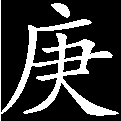
\includegraphics[width=3mm]{../Images/00004}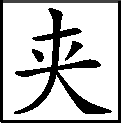
\includegraphics[width=3mm]{../Images/00012}\footnotesize \kaishu 是月初旬起更时也。}鸳鸯又不曾有个作伴的,也不曾提灯笼,独自一个,脚步又轻,所以该班的人皆不理会。偏生又要小解,因下了甬路,寻微草处,行至一湖山石后大桂树阴下来。{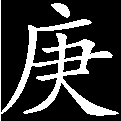
\includegraphics[width=3mm]{../Images/00004}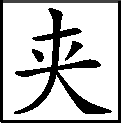
\includegraphics[width=3mm]{../Images/00012}\footnotesize \kaishu 是八月,随笔点景。}

刚转过石后,只听一阵衣衫响,吓了一惊不小。定睛一看,只见是两个人在那里,见他来了,便想往石后树丛藏躲。鸳鸯眼尖,趁月色见准一个穿红裙子、梳鬅头、高大丰壮身材的,{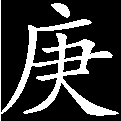
\includegraphics[width=3mm]{../Images/00004}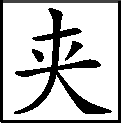
\includegraphics[width=3mm]{../Images/00012}\footnotesize \kaishu 是月下所见之像,故不写至容貌也。}是迎春房里的司棋。鸳鸯只当他和别的女孩子也在此方便,见自己来了,故意藏躲恐吓着耍,{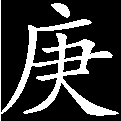
\includegraphics[width=3mm]{../Images/00004}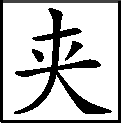
\includegraphics[width=3mm]{../Images/00012}\footnotesize \kaishu 此见是女儿们常事,观书者自亦为如此。}因便笑叫道:“司棋你不快出来,吓着我,我就喊起来当贼拿了。这么大丫头了,没个黑家白日的只是顽不够。”这本是鸳鸯的戏语,叫他出来。谁知他贼人胆虚,{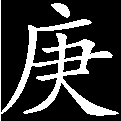
\includegraphics[width=3mm]{../Images/00004}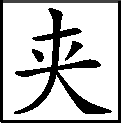
\includegraphics[width=3mm]{../Images/00012}\footnotesize \kaishu 更奇,不知后为何事。}只当鸳鸯已看见他的首尾了,生恐叫喊起来使众人知觉更不好,且素日鸳鸯又和自己亲厚不比别人,便从树后跑出来,一把拉住鸳鸯,便双膝跪下,只说:“好姐姐,千万别嚷!”{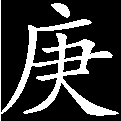
\includegraphics[width=3mm]{../Images/00004}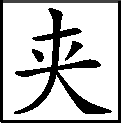
\includegraphics[width=3mm]{../Images/00012}\footnotesize \kaishu 奇甚!}鸳鸯反不知因何,忙拉他起来,笑问道:“这是怎么说?”司棋满脸红胀,又流下泪来。

鸳鸯再一回想,那一个人影恍惚像个小厮,心下便猜疑了八九,{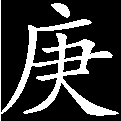
\includegraphics[width=3mm]{../Images/00004}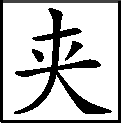
\includegraphics[width=3mm]{../Images/00012}\footnotesize \kaishu 是聪敏女儿,妙!}自己反羞的面红耳赤,{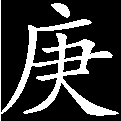
\includegraphics[width=3mm]{../Images/00004}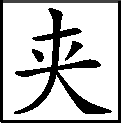
\includegraphics[width=3mm]{../Images/00012}\footnotesize \kaishu 是娇贵女儿,笔笔皆到。}又怕起来。因定了一会,忙悄问:“那个是谁?”司棋复跪下道:“是我姑舅兄弟。”{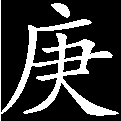
\includegraphics[width=3mm]{../Images/00004}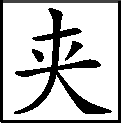
\includegraphics[width=3mm]{../Images/00012}\footnotesize \kaishu 妙!}鸳鸯啐了一口,道:“要死,要死。”{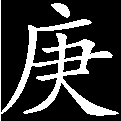
\includegraphics[width=3mm]{../Images/00004}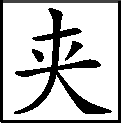
\includegraphics[width=3mm]{../Images/00012}\footnotesize \kaishu 如见其面,如闻其声。}司棋又回头悄道:“你不用藏着,姐姐已看见了,快出来磕头。”那小厮听了,只得也从树后爬出来,磕头如捣蒜。鸳鸯忙要回身,司棋拉住苦求,哭道:“我们的性命,都在姐姐身上,只求姐姐超生要紧!”鸳鸯道:“你放心,我横竖不告诉一个人就是了。”一语未了,只听角门上有人说道:“金姑娘已出去了,角门上锁罢。”鸳鸯正被司棋拉住,不得脱身,听见如此说,便接声道:“我在这里有事,且略住手,我出来了。”司棋听了,只得松手让他去了------

{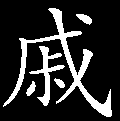
\includegraphics[width=3mm]{../Images/00005}\kaishu 总评:叙一番灯火未息,门户未关。叙一番赵姨失体,费婆憋气。叙一番林家托大,周家献勤。叙一番凤姐灰心,鸳鸯传信。非为本文渲染,全为下文引逗,良工苦心,可谓惨淡经营。}

{\kaishu 司棋事从鸳鸯误吓得来,是善周全处。方与鸳鸯前后行景不致矛盾。一何精细如此。}
